\section{Results}

The results present representation quality, original development selection and confirmatory assessment before the separate post-hoc sensitivity and transfer findings.

\subsection{Representation Quality and Capacity}

Table~\ref{tab:som} summarises the 70-epoch experiment, reporting validation CQE with sample standard deviations alongside validation TE and training-BMU occupancy. Figure~\ref{fig:representation} shows the capacity trends with five-seed standard-deviation error bars. Log-standard preprocessing gave lower validation CQE at every capacity, reaching 0.1412 on the largest map compared with 0.1665 under standard preprocessing. Lower contextual distance indicated closer codebook fit within the transformed spaces, without establishing a transformation-independent advantage.

\begin{table}[!ht]
\caption{Development representation diagnostics}
\label{tab:som}
\centering
\footnotesize
\setlength{\tabcolsep}{3pt}
\begin{tabular}{@{}llrrr@{}}
\toprule
Representation & Map & Validation CQE & TE & Occupancy (\%) \\
\midrule
Standard & $8\times8$ & 0.4116 $\pm$ 0.0080 & 0.114 & 92.8 \\
Standard & $16\times16$ & 0.2548 $\pm$ 0.0019 & 0.151 & 87.2 \\
Standard & $24\times24$ & 0.1981 $\pm$ 0.0021 & 0.150 & 82.7 \\
Standard & $32\times32$ & 0.1665 $\pm$ 0.0019 & 0.145 & 80.4 \\
Log-standard & $8\times8$ & 0.3130 $\pm$ 0.0019 & 0.081 & 93.4 \\
Log-standard & $16\times16$ & 0.2057 $\pm$ 0.0009 & 0.111 & 87.7 \\
Log-standard & $24\times24$ & 0.1625 $\pm$ 0.0012 & 0.129 & 85.8 \\
Log-standard & $32\times32$ & 0.1412 $\pm$ 0.0005 & 0.154 & 84.6 \\
\bottomrule

\end{tabular}
\end{table}

\begin{figure*}[!t]
\centering
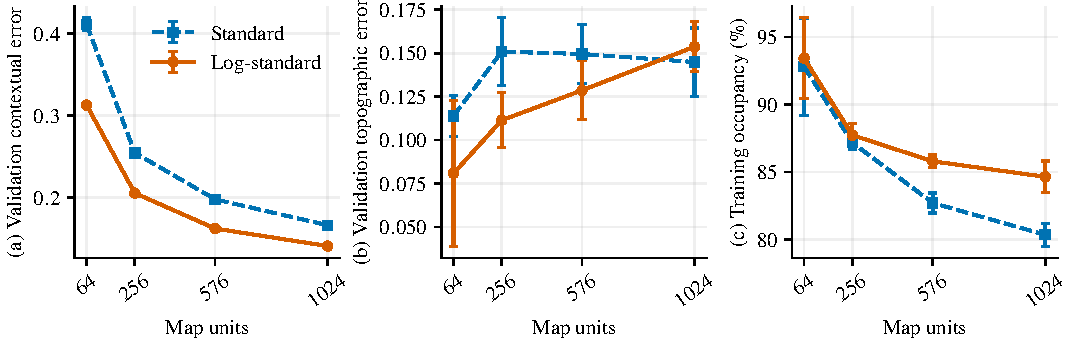
\includegraphics[width=\textwidth]{representation.pdf}
\caption{Development representation diagnostics across map capacity}
\label{fig:representation}
\end{figure*}

Increasing capacity reduced CQE with diminishing returns, as the log-standard improvement from $8\times8$ to $16\times16$ exceeded the improvement from $24\times24$ to $32\times32$. Occupancy fell and validation TE increased, while the largest standard map preserved lower TE than the largest log-standard map. Log-standard preprocessing therefore improved contextual fit without improving every diagnostic, and topology varied more across seeds than CQE. For the log-standard $8\times8$ map, TE had standard deviation 0.042 around a mean of 0.081.

Fixed-radius refinement flattened the convergence histories, with mean validation QE changes below 0.03\% in magnitude during the last 10 updates for every log-standard capacity. Final mean movement on the largest log-standard map was approximately 0.0009 transformed Euclidean units, supporting practical stabilisation without establishing an exact fixed point.

Figure~\ref{fig:geometry} presents an unlabelled development map selected by median original development performance within the seed hierarchy. The neighbour-distance panel averages distances to edge-sharing codebook vectors at each unit, while training hits use a logarithmic scale. Duration and source bytes were predeclared semantic features, shown in transformed coordinates centred around zero. Together, the panels illustrate unequal support and spatial variation without class overlays.

\begin{figure*}[!t]
\centering
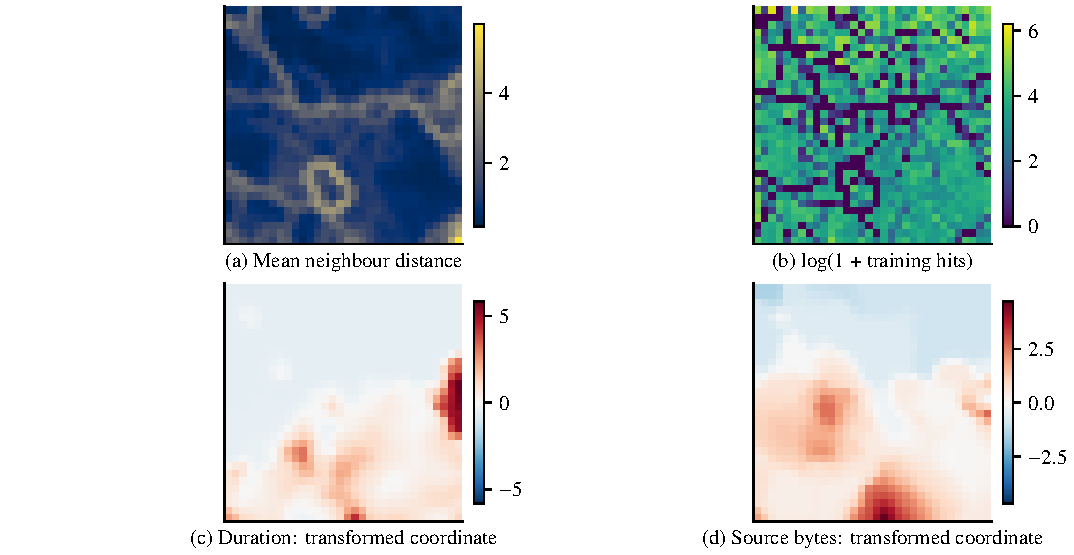
\includegraphics[width=\textwidth]{geometry.pdf}
\caption{Unlabelled development geometry and component planes}
\label{fig:geometry}
\end{figure*}

\subsection{Original Development Selection}

The original grid selected log-standard $32\times32$ geometry with 40 hit-weighted clusters and full correction, achieving validation macro $F_1$ of 0.3164 with SOM standard deviation 0.0049. Intermediate and compact maps achieved 0.3066 and 0.2979, respectively, so macro $F_1$ selection favoured the largest map despite higher balanced accuracy for the intermediate map.

At the selected capacity and cluster count, majority mapping achieved macro $F_1$ of 0.2654 and accuracy of 0.6932. Full correction raised macro $F_1$ to 0.3164 but lowered accuracy to 0.5851, while mean predicted-class coverage increased from 4.4 to 9.92. Corrected Worms recall reached approximately 0.714, yet 387 false positives accompanied only seven true validation cases. Broader class coverage therefore did not establish adequate precision.

Under otherwise matching corrected settings, uniform weighting achieved macro $F_1$ of 0.3026, below the training-hit-weighted result. Performance was still rising at 40 clusters, but the procedure was frozen at the declared boundary before confirmatory assessment.

\subsection{Confirmatory Assessment}

The 40-cluster procedure achieved pooled assessment macro $F_1$ of \ConfirmF, with SOM-level standard deviation 0.0060 and mean within-SOM clustering standard deviation 0.0078. The estimates remained the primary confirmatory results, compared with same-fold macro $F_1$ of \NeighbourF\ for kNN and \TreeF\ for the tree. The tree achieved the highest balanced accuracy, whereas kNN achieved the highest accuracy and weighted $F_1$.

Across 25 fold-specific SOMs, mean training and held-out CQE remained close at approximately 0.1365 and 0.1384, with corresponding TE of 0.1256 and 0.1337. Comparable diagnostics supported geometric transfer to unseen groups despite weak classification performance. Every cluster had training support, ruling out unsupported-cluster fallback as a source of classification errors.

Rare-class recall nevertheless accompanied extensive false positives, particularly for the 139 assessment Worms observations. Worms recall averaged 0.707 but precision only 0.013, with approximately 98 true positives and 7,205 false positives per replicate. Shellcode showed a similar imbalance, with recall 0.540 and precision 0.030, motivating the subsequent sensitivity study.

\subsection{Post-Hoc Development Sensitivity}

Figure~\ref{fig:sensitivity} shows all 50 nested means from varying granularity and correction on unchanged SOMs. A dashed boundary separates the first extension from the final higher-granularity extension. Macro $F_1$ increased with cluster count at every tested correction strength, and partial correction gave the highest mean at every count. The best $\alpha$ was 0.75 at 60, 80 and 100 clusters, and 0.5 elsewhere.

\begin{figure}[!ht]
\centering
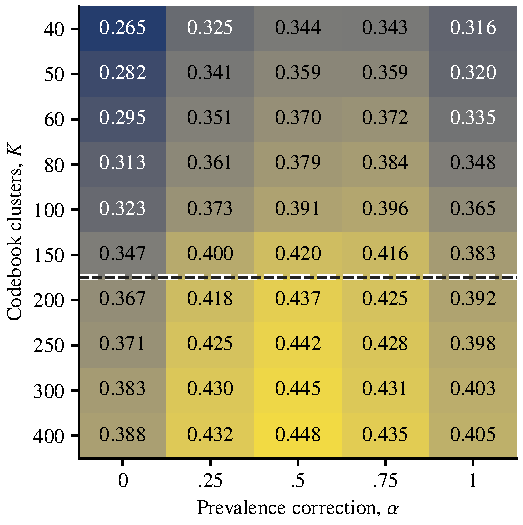
\includegraphics[width=\columnwidth]{sensitivity.pdf}
\caption{Post-hoc development sensitivity to granularity and correction}
\label{fig:sensitivity}
\end{figure}

At $\alpha=0.5$, the 150-cluster procedure achieved development macro $F_1$ of 0.4196, a gain of 0.1032 over the frozen procedure. The final extension reached 0.4475 at 400 clusters, although gains at fixed $\alpha=0.5$ fell from 0.0284 for 100--150 clusters to 0.0026 for 300--400 clusters. The diminishing gains did not establish a plateau or global optimum.

Figure~\ref{fig:fragmentation} relates classification to fragmentation at fixed $\alpha=0.5$, with SOM-level standard-deviation error bars. Singleton fractions count clusters containing a single unit, while tiny fractions count clusters containing fewer than 10 training observations. Silhouette fell as singleton clusters increased, reaching singleton and tiny fractions of approximately 27.5\% and 2.5\% at 400 clusters. All clusters retained positive support, so the predictive gains concerned finer partitions of the same codebook without changing SOM quantisation.

\begin{figure}[!t]
\centering
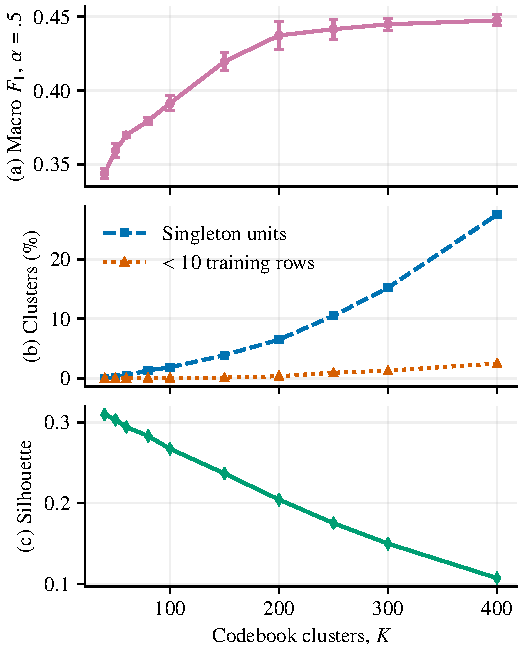
\includegraphics[width=\columnwidth]{fragmentation.pdf}
\caption{Post-hoc development performance and codebook fragmentation}
\label{fig:fragmentation}
\end{figure}

\subsection{Post-Hoc Assessment Transfer and Class Effects}

Table~\ref{tab:overall} compares all five procedures on shared folds, with macro $F_1$ uncertainty denoting sample standard deviation across five SOM-level means. Figure~\ref{fig:transfer} compares development and assessment performance, distinguishing the confirmatory 40-cluster result from the post-hoc larger-cluster results. Development gains transferred to the already-viewed assessment block, but the transfer did not provide independent confirmation.

\begin{table*}[!t]
\caption{Assessment performance on the shared outer folds}
\label{tab:overall}
\centering
\begin{tabular}{@{}llrrrr@{}}
\toprule
Procedure & Status & Macro $F_1$ & Balanced accuracy & Accuracy & Weighted $F_1$ \\
\midrule
SOM K40 & Confirmatory & 0.3237 $\pm$ 0.0060 & 0.4611 & 0.5868 & 0.6455 \\
SOM K150 & Post-hoc & 0.4335 $\pm$ 0.0021 & 0.4569 & 0.7178 & 0.7352 \\
SOM K400 & Post-hoc & 0.4584 $\pm$ 0.0017 & 0.4915 & 0.7307 & 0.7469 \\
kNN & Frozen baseline & 0.5233 & 0.5060 & 0.8008 & 0.7957 \\
Tree & Frozen baseline & 0.5834 & 0.6661 & 0.7566 & 0.7821 \\
\bottomrule

\end{tabular}
\end{table*}

\begin{figure}[!t]
\centering
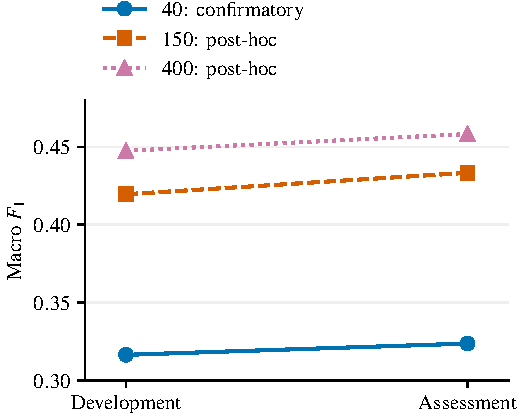
\includegraphics[width=\columnwidth]{transfer.pdf}
\caption{Development and assessment macro $F_1$ for the map-derived procedures}
\label{fig:transfer}
\end{figure}

At fixed $\alpha=0.5$, the 400-cluster procedure exceeded the 150-cluster procedure by 0.0250 assessment macro $F_1$, with positive differences across all 25 paired stochastic replicates. The paired group-bootstrap interval was [0.0233, 0.0266], while the gain over the confirmatory procedure was 0.1347 with interval [0.1308, 0.1384]. Both intervals described resampling sensitivity under the post-hoc procedures.

Figure~\ref{fig:classes} retains all 10 classes, showing improvements for Reconnaissance and DoS relative to the coarse, fully corrected procedure. Generic maintained high class $F_1$, while finer clustering improved Shellcode without reaching either supervised baseline. Backdoor and Analysis continued to have low class $F_1$.

\begin{figure*}[!t]
\centering
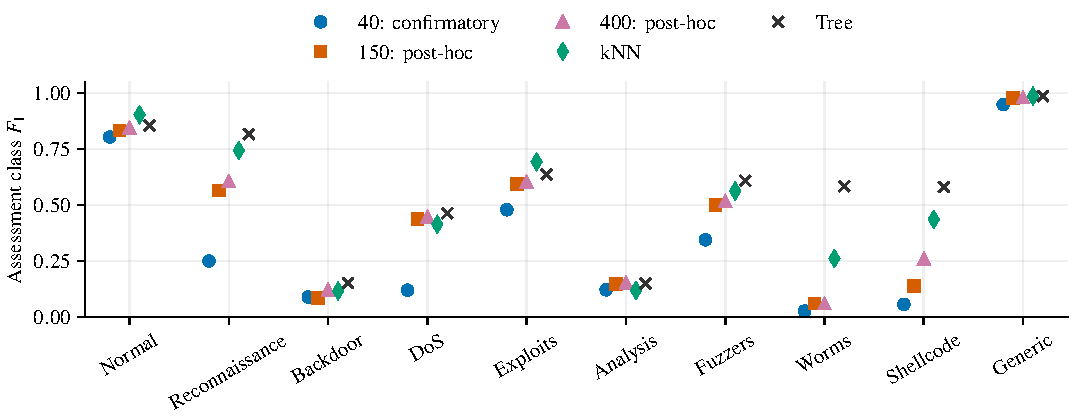
\includegraphics[width=\textwidth]{classes.pdf}
\caption{Class-specific assessment $F_1$ on the shared outer folds}
\label{fig:classes}
\end{figure*}

Table~\ref{tab:rare} reports precision, recall and false-positive counts for four rare classes, with fractional counts obtained by averaging 25 integer confusion matrices. Finer clustering with partial correction sharply reduced Worms false positives but also reduced recall, giving approximately 180 false positives and recall 0.072 at 150 clusters. Increasing to 400 clusters raised recall to 0.127 alongside approximately 451 false positives, lowering precision and leaving Worms $F_1$ near 0.059 under both procedures. Weak recall across 139 assessment cases therefore extended beyond the uncertainty of the seven-case development sample.

\begin{table*}[!t]
\caption{Rare-class assessment performance of the map-derived procedures}
\label{tab:rare}
\centering
\begin{tabular}{@{}llrrrrrr@{}}
\toprule
Class (true support) & $K$ / $\alpha$ & Precision & Recall & $F_1$ & True positives & False positives & False negatives \\
\midrule
Backdoor (1,864) & 40 / 1 & 0.049 & 0.511 & 0.089 & 952.2 & 18,699.8 & 911.8 \\
Backdoor (1,864) & 150 / .5 & 0.115 & 0.070 & 0.084 & 130.1 & 1,009.9 & 1733.9 \\
Backdoor (1,864) & 400 / .5 & 0.125 & 0.118 & 0.121 & 220.8 & 1,557.9 & 1643.2 \\
\addlinespace[2pt]
Analysis (2,141) & 40 / 1 & 0.107 & 0.152 & 0.121 & 325.0 & 2,999.9 & 1816.0 \\
Analysis (2,141) & 150 / .5 & 0.210 & 0.112 & 0.146 & 240.6 & 909.8 & 1900.4 \\
Analysis (2,141) & 400 / .5 & 0.221 & 0.113 & 0.150 & 242.8 & 857.6 & 1898.2 \\
\addlinespace[2pt]
Worms (139) & 40 / 1 & 0.013 & 0.707 & 0.026 & 98.3 & 7,205.3 & 40.7 \\
Worms (139) & 150 / .5 & 0.058 & 0.072 & 0.060 & 10.0 & 179.6 & 129.0 \\
Worms (139) & 400 / .5 & 0.039 & 0.127 & 0.059 & 17.6 & 451.4 & 121.4 \\
\addlinespace[2pt]
Shellcode (1,208) & 40 / 1 & 0.030 & 0.540 & 0.056 & 652.8 & 21,552.8 & 555.2 \\
Shellcode (1,208) & 150 / .5 & 0.147 & 0.137 & 0.138 & 164.9 & 981.6 & 1043.1 \\
Shellcode (1,208) & 400 / .5 & 0.220 & 0.315 & 0.259 & 380.4 & 1,353.4 & 827.6 \\
\addlinespace[2pt]
\bottomrule

\end{tabular}
\end{table*}

Assessment-fold codebooks reproduced the fragmentation trend, with singleton clusters increasing from 4.46\% at $K=150$ to 27.53\% at $K=400$ as mean silhouette fell from 0.241 to 0.108. Held-out purity rose from 0.754 to 0.768, but NMI and ARI fell, showing that improved prediction did not imply improvement under every structural measure.

The 400-cluster procedure remained below both supervised baselines, with a macro $F_1$ gap to kNN of $-0.0649$ and paired interval [$-0.0761$, $-0.0527$]. The tree gap was $-0.1250$, with interval [$-0.1350$, $-0.1147$], retaining the descriptive, post-hoc interpretation.